
%% bare_jrnl.tex
%% V1.4b
%% 2015/08/26
%% by Michael Shell
%% see http://www.michaelshell.org/
%% for current contact information.
%%
%% This is a skeleton file demonstrating the use of IEEEtran.cls
%% (requires IEEEtran.cls version 1.8b or later) with an IEEE
%% journal paper.
%%
%% Support sites:
%% http://www.michaelshell.org/tex/ieeetran/
%% http://www.ctan.org/pkg/ieeetran
%% and
%% http://www.ieee.org/

%%*************************************************************************
%% Legal Notice:
%% This code is offered as-is without any warranty either expressed or
%% implied; without even the implied warranty of MERCHANTABILITY or
%% FITNESS FOR A PARTICULAR PURPOSE! 
%% User assumes all risk.
%% In no event shall the IEEE or any contributor to this code be liable for
%% any damages or losses, including, but not limited to, incidental,
%% consequential, or any other damages, resulting from the use or misuse
%% of any information contained here.
%%
%% All comments are the opinions of their respective authors and are not
%% necessarily endorsed by the IEEE.
%%
%% This work is distributed under the LaTeX Project Public License (LPPL)
%% ( http://www.latex-project.org/ ) version 1.3, and may be freely used,
%% distributed and modified. A copy of the LPPL, version 1.3, is included
%% in the base LaTeX documentation of all distributions of LaTeX released
%% 2003/12/01 or later.
%% Retain all contribution notices and credits.
%% ** Modified files should be clearly indicated as such, including  **
%% ** renaming them and changing author support contact information. **
%%*************************************************************************


% *** Authors should verify (and, if needed, correct) their LaTeX system  ***
% *** with the testflow diagnostic prior to trusting their LaTeX platform ***
% *** with production work. The IEEE's font choices and paper sizes can   ***
% *** trigger bugs that do not appear when using other class files.       ***                          ***
% The testflow support page is at:
% http://www.michaelshell.org/tex/testflow/



\documentclass[journal]{IEEEtran}
%
% If IEEEtran.cls has not been installed into the LaTeX system files,
% manually specify the path to it like:
% \documentclass[journal]{../sty/IEEEtran}

\usepackage{amsfonts}
\usepackage{CJK}
\usepackage{amsmath}
\usepackage{bm}
\usepackage{multirow}
\usepackage{amssymb}
\usepackage{latexsym}
\usepackage{makecell}
\usepackage{booktabs}
\usepackage{fancybox}
\usepackage{array}

\usepackage{algorithm}
\usepackage{algorithmicx}
\usepackage{algpseudocode}




% Some very useful LaTeX packages include:
% (uncomment the ones you want to load)


% *** MISC UTILITY PACKAGES ***
%
%\usepackage{ifpdf}
% Heiko Oberdiek's ifpdf.sty is very useful if you need conditional
% compilation based on whether the output is pdf or dvi.
% usage:
% \ifpdf
%   % pdf code
% \else
%   % dvi code
% \fi
% The latest version of ifpdf.sty can be obtained from:
% http://www.ctan.org/pkg/ifpdf
% Also, note that IEEEtran.cls V1.7 and later provides a builtin
% \ifCLASSINFOpdf conditional that works the same way.
% When switching from latex to pdflatex and vice-versa, the compiler may
% have to be run twice to clear warning/error messages.






% *** CITATION PACKAGES ***
%
%\usepackage{cite}
% cite.sty was written by Donald Arseneau
% V1.6 and later of IEEEtran pre-defines the format of the cite.sty package
% \cite{} output to follow that of the IEEE. Loading the cite package will
% result in citation numbers being automatically sorted and properly
% "compressed/ranged". e.g., [1], [9], [2], [7], [5], [6] without using
% cite.sty will become [1], [2], [5]--[7], [9] using cite.sty. cite.sty's
% \cite will automatically add leading space, if needed. Use cite.sty's
% noadjust option (cite.sty V3.8 and later) if you want to turn this off
% such as if a citation ever needs to be enclosed in parenthesis.
% cite.sty is already installed on most LaTeX systems. Be sure and use
% version 5.0 (2009-03-20) and later if using hyperref.sty.
% The latest version can be obtained at:
% http://www.ctan.org/pkg/cite
% The documentation is contained in the cite.sty file itself.






% *** GRAPHICS RELATED PACKAGES ***
%
\ifCLASSINFOpdf
   \usepackage[pdftex]{graphicx}
  % declare the path(s) where your graphic files are
   \graphicspath{{../pdf/}{../jpeg/}}
  % and their extensions so you won't have to specify these with
  % every instance of \includegraphics
   \DeclareGraphicsExtensions{.pdf,.jpeg,.png}
\else
  % or other class option (dvipsone, dvipdf, if not using dvips). graphicx
  % will default to the driver specified in the system graphics.cfg if no
  % driver is specified.
   \usepackage[dvips]{graphicx}
  % declare the path(s) where your graphic files are
   \graphicspath{{../eps/}}
  % and their extensions so you won't have to specify these with
  % every instance of \includegraphics
  % \DeclareGraphicsExtensions{.eps}
\fi
% graphicx was written by David Carlisle and Sebastian Rahtz. It is
% required if you want graphics, photos, etc. graphicx.sty is already
% installed on most LaTeX systems. The latest version and documentation
% can be obtained at: 
% http://www.ctan.org/pkg/graphicx
% Another good source of documentation is "Using Imported Graphics in
% LaTeX2e" by Keith Reckdahl which can be found at:
% http://www.ctan.org/pkg/epslatex
%
% latex, and pdflatex in dvi mode, support graphics in encapsulated
% postscript (.eps) format. pdflatex in pdf mode supports graphics
% in .pdf, .jpeg, .png and .mps (metapost) formats. Users should ensure
% that all non-photo figures use a vector format (.eps, .pdf, .mps) and
% not a bitmapped formats (.jpeg, .png). The IEEE frowns on bitmapped formats
% which can result in "jaggedy"/blurry rendering of lines and letters as
% well as large increases in file sizes.
%
% You can find documentation about the pdfTeX application at:
% http://www.tug.org/applications/pdftex





% *** MATH PACKAGES ***
%
%\usepackage{amsmath}
% A popular package from the American Mathematical Society that provides
% many useful and powerful commands for dealing with mathematics.
%
% Note that the amsmath package sets \interdisplaylinepenalty to 10000
% thus preventing page breaks from occurring within multiline equations. Use:
%\interdisplaylinepenalty=2500
% after loading amsmath to restore such page breaks as IEEEtran.cls normally
% does. amsmath.sty is already installed on most LaTeX systems. The latest
% version and documentation can be obtained at:
% http://www.ctan.org/pkg/amsmath





% *** SPECIALIZED LIST PACKAGES ***
%
%\usepackage{algorithmic}
% algorithmic.sty was written by Peter Williams and Rogerio Brito.
% This package provides an algorithmic environment fo describing algorithms.
% You can use the algorithmic environment in-text or within a figure
% environment to provide for a floating algorithm. Do NOT use the algorithm
% floating environment provided by algorithm.sty (by the same authors) or
% algorithm2e.sty (by Christophe Fiorio) as the IEEE does not use dedicated
% algorithm float types and packages that provide these will not provide
% correct IEEE style captions. The latest version and documentation of
% algorithmic.sty can be obtained at:
% http://www.ctan.org/pkg/algorithms
% Also of interest may be the (relatively newer and more customizable)
% algorithmicx.sty package by Szasz Janos:
% http://www.ctan.org/pkg/algorithmicx




% *** ALIGNMENT PACKAGES ***
%
%\usepackage{array}
% Frank Mittelbach's and David Carlisle's array.sty patches and improves
% the standard LaTeX2e array and tabular environments to provide better
% appearance and additional user controls. As the default LaTeX2e table
% generation code is lacking to the point of almost being broken with
% respect to the quality of the end results, all users are strongly
% advised to use an enhanced (at the very least that provided by array.sty)
% set of table tools. array.sty is already installed on most systems. The
% latest version and documentation can be obtained at:
% http://www.ctan.org/pkg/array


% IEEEtran contains the IEEEeqnarray family of commands that can be used to
% generate multiline equations as well as matrices, tables, etc., of high
% quality.




% *** SUBFIGURE PACKAGES ***
%\ifCLASSOPTIONcompsoc
%  \usepackage[caption=false,font=normalsize,labelfont=sf,textfont=sf]{subfig}
%\else
%  \usepackage[caption=false,font=footnotesize]{subfig}
%\fi
% subfig.sty, written by Steven Douglas Cochran, is the modern replacement
% for subfigure.sty, the latter of which is no longer maintained and is
% incompatible with some LaTeX packages including fixltx2e. However,
% subfig.sty requires and automatically loads Axel Sommerfeldt's caption.sty
% which will override IEEEtran.cls' handling of captions and this will result
% in non-IEEE style figure/table captions. To prevent this problem, be sure
% and invoke subfig.sty's "caption=false" package option (available since
% subfig.sty version 1.3, 2005/06/28) as this is will preserve IEEEtran.cls
% handling of captions.
% Note that the Computer Society format requires a larger sans serif font
% than the serif footnote size font used in traditional IEEE formatting
% and thus the need to invoke different subfig.sty package options depending
% on whether compsoc mode has been enabled.
%
% The latest version and documentation of subfig.sty can be obtained at:
% http://www.ctan.org/pkg/subfig




% *** FLOAT PACKAGES ***
%
%\usepackage{fixltx2e}
% fixltx2e, the successor to the earlier fix2col.sty, was written by
% Frank Mittelbach and David Carlisle. This package corrects a few problems
% in the LaTeX2e kernel, the most notable of which is that in current
% LaTeX2e releases, the ordering of single and double column floats is not
% guaranteed to be preserved. Thus, an unpatched LaTeX2e can allow a
% single column figure to be placed prior to an earlier double column
% figure.
% Be aware that LaTeX2e kernels dated 2015 and later have fixltx2e.sty's
% corrections already built into the system in which case a warning will
% be issued if an attempt is made to load fixltx2e.sty as it is no longer
% needed.
% The latest version and documentation can be found at:
% http://www.ctan.org/pkg/fixltx2e


%\usepackage{stfloats}
% stfloats.sty was written by Sigitas Tolusis. This package gives LaTeX2e
% the ability to do double column floats at the bottom of the page as well
% as the top. (e.g., "\begin{figure*}[!b]" is not normally possible in
% LaTeX2e). It also provides a command:
%\fnbelowfloat
% to enable the placement of footnotes below bottom floats (the standard
% LaTeX2e kernel puts them above bottom floats). This is an invasive package
% which rewrites many portions of the LaTeX2e float routines. It may not work
% with other packages that modify the LaTeX2e float routines. The latest
% version and documentation can be obtained at:
% http://www.ctan.org/pkg/stfloats
% Do not use the stfloats baselinefloat ability as the IEEE does not allow
% \baselineskip to stretch. Authors submitting work to the IEEE should note
% that the IEEE rarely uses double column equations and that authors should try
% to avoid such use. Do not be tempted to use the cuted.sty or midfloat.sty
% packages (also by Sigitas Tolusis) as the IEEE does not format its papers in
% such ways.
% Do not attempt to use stfloats with fixltx2e as they are incompatible.
% Instead, use Morten Hogholm'a dblfloatfix which combines the features
% of both fixltx2e and stfloats:
%
% \usepackage{dblfloatfix}
% The latest version can be found at:
% http://www.ctan.org/pkg/dblfloatfix




%\ifCLASSOPTIONcaptionsoff
%  \usepackage[nomarkers]{endfloat}
% \let\MYoriglatexcaption\caption
% \renewcommand{\caption}[2][\relax]{\MYoriglatexcaption[#2]{#2}}
%\fi
% endfloat.sty was written by James Darrell McCauley, Jeff Goldberg and 
% Axel Sommerfeldt. This package may be useful when used in conjunction with 
% IEEEtran.cls'  captionsoff option. Some IEEE journals/societies require that
% submissions have lists of figures/tables at the end of the paper and that
% figures/tables without any captions are placed on a page by themselves at
% the end of the document. If needed, the draftcls IEEEtran class option or
% \CLASSINPUTbaselinestretch interface can be used to increase the line
% spacing as well. Be sure and use the nomarkers option of endfloat to
% prevent endfloat from "marking" where the figures would have been placed
% in the text. The two hack lines of code above are a slight modification of
% that suggested by in the endfloat docs (section 8.4.1) to ensure that
% the full captions always appear in the list of figures/tables - even if
% the user used the short optional argument of \caption[]{}.
% IEEE papers do not typically make use of \caption[]'s optional argument,
% so this should not be an issue. A similar trick can be used to disable
% captions of packages such as subfig.sty that lack options to turn off
% the subcaptions:
% For subfig.sty:
% \let\MYorigsubfloat\subfloat
% \renewcommand{\subfloat}[2][\relax]{\MYorigsubfloat[]{#2}}
% However, the above trick will not work if both optional arguments of
% the \subfloat command are used. Furthermore, there needs to be a
% description of each subfigure *somewhere* and endfloat does not add
% subfigure captions to its list of figures. Thus, the best approach is to
% avoid the use of subfigure captions (many IEEE journals avoid them anyway)
% and instead reference/explain all the subfigures within the main caption.
% The latest version of endfloat.sty and its documentation can obtained at:
% http://www.ctan.org/pkg/endfloat
%
% The IEEEtran \ifCLASSOPTIONcaptionsoff conditional can also be used
% later in the document, say, to conditionally put the References on a 
% page by themselves.




% *** PDF, URL AND HYPERLINK PACKAGES ***
%
%\usepackage{url}
% url.sty was written by Donald Arseneau. It provides better support for
% handling and breaking URLs. url.sty is already installed on most LaTeX
% systems. The latest version and documentation can be obtained at:
% http://www.ctan.org/pkg/url
% Basically, \url{my_url_here}.




% *** Do not adjust lengths that control margins, column widths, etc. ***
% *** Do not use packages that alter fonts (such as pslatex).         ***
% There should be no need to do such things with IEEEtran.cls V1.6 and later.
% (Unless specifically asked to do so by the journal or conference you plan
% to submit to, of course. )


% correct bad hyphenation here
\hyphenation{op-tical net-works semi-conduc-tor}


\begin{document}
%
% paper title
% Titles are generally capitalized except for words such as a, an, and, as,
% at, but, by, for, in, nor, of, on, or, the, to and up, which are usually
% not capitalized unless they are the first or last word of the title.
% Linebreaks \\ can be used within to get better formatting as desired.
% Do not put math or special symbols in the title.
\title{XXX Vehicle-based Crowd Sensing with Schedulable Trajectory  XXX }
%
%
% author names and IEEE memberships
% note positions of commas and nonbreaking spaces ( ~ ) LaTeX will not break
% a structure at a ~ so this keeps an author's name from being broken across
% two lines.
% use \thanks{} to gain access to the first footnote area
% a separate \thanks must be used for each paragraph as LaTeX2e's \thanks
% was not built to handle multiple paragraphs
%

\author{Name1,~Name2,~\IEEEmembership{Member,~IEEE,}
	    Name3,~and~Name4,~\IEEEmembership{Member,~IEEE}
       % <-this % stops a space
\thanks{Sheng Zeng, Chaowei Wang, Cai Qin, and Weidong Wang are with School of Electronic Engineering, Beijing University of Posts and Telecommunications, Beijing, China, 100876, (e-mail: \{zengsheng, wangchaowei, qincai, wangweidong\}@bupt.edu.cn).}% <-this % stops a space
% <-this % stops a space
\thanks{Manuscript received XXXX XX, 2017; revised XXXX XX, 2017.}}

% note the % following the last \IEEEmembership and also \thanks - 
% these prevent an unwanted space from occurring between the last author name
% and the end of the author line. i.e., if you had this:
% 
% \author{....lastname \thanks{...} \thanks{...} }
%                     ^------------^------------^----Do not want these spaces!
%
% a space would be appended to the last name and could cause every name on that
% line to be shifted left slightly. This is one of those "LaTeX things". For
% instance, "\textbf{A} \textbf{B}" will typeset as "A B" not "AB". To get
% "AB" then you have to do: "\textbf{A}\textbf{B}"
% \thanks is no different in this regard, so shield the last } of each \thanks
% that ends a line with a % and do not let a space in before the next \thanks.
% Spaces after \IEEEmembership other than the last one are OK (and needed) as
% you are supposed to have spaces between the names. For what it is worth,
% this is a minor point as most people would not even notice if the said evil
% space somehow managed to creep in.



% The paper headers
%%\markboth{Journal of \LaTeX\ Class Files,~Vol.~14, No.~8, August~2015}%
%%{Shell \MakeLowercase{\textit{et al.}}: Bare Demo of IEEEtran.cls for IEEE Journals}
% The only time the second header will appear is for the odd numbered pages
% after the title page when using the twoside option.
% 
% *** Note that you probably will NOT want to include the author's ***
% *** name in the headers of peer review papers.                   ***
% You can use \ifCLASSOPTIONpeerreview for conditional compilation here if
% you desire.




% If you want to put a publisher's ID mark on the page you can do it like
% this:
%\IEEEpubid{0000--0000/00\$00.00~\copyright~2015 IEEE}
% Remember, if you use this you must call \IEEEpubidadjcol in the second
% column for its text to clear the IEEEpubid mark.



% use for special paper notices
%\IEEEspecialpapernotice{(Invited Paper)}




% make the title area
\maketitle

% As a general rule, do not put math, special symbols or citations
% in the abstract or keywords.
\begin{abstract}
Mobile crowd sensing has been becoming a prospective paradigm with smartphone, which can collect ubiquitous data easily in large-scale city. Nowadays, public transport buses are mostly widely used and affordable transport vehicle in many urban. A buses embedded with substantial sensors also can be adopted as participator in crowd sensing. However, distinct from smartphones, the trajectory of bus is scheduled and whose location is predicted, which opens up a new opportunities to achieve high quality crowd sensing. A high quality of a crowd sensing network highly depends on the spatial-temporal coverage of sensing data, therefore, based on the predictable trajectory of vehicles, we design a novel model and present an approximation algorithm to select vehicles to participate in urban sensing for maximizing spatiotemporal coverage with constraint sensing reward. We theoretically prove that the selection of vehicles problem is NP-hard, the proposed algorithm can achieve a performance guarantee no less than $\left ( 1-e^{-1} \right )$ of theoretical optimum. The performance of our algorithm is stimulated with real T-Drive trajectory dataset. The results shows that our algorithm achieves a good coverage closer to optimum and outperform some exiting alternative algorithms.
\end{abstract}

% Note that keywords are not normally used for peerreview papers.
\begin{IEEEkeywords}
Mobile crowd sensing, spatial temporal coverage, approximation algorithm, performance guarantee.
\end{IEEEkeywords}






% For peer review papers, you can put extra information on the cover
% page as needed:
% \ifCLASSOPTIONpeerreview
% \begin{center} \bfseries EDICS Category: 3-BBND \end{center}
% \fi
%
% For peerreview papers, this IEEEtran command inserts a page break and
% creates the second title. It will be ignored for other modes.
\IEEEpeerreviewmaketitle



\section{Introduction}

% The very first letter is a 2 line initial drop letter followed
% by the rest of the first word in caps.
% 
% form to use if the first word consists of a single letter:
% \IEEEPARstart{A}{demo} file is ....
% 
% form to use if you need the single drop letter followed by
% normal text (unknown if ever used by the IEEE):
% \IEEEPARstart{A}{}demo file is ....
% 
% Some journals put the first two words in caps:
% \IEEEPARstart{T}{his demo} file is ....
% 
% Here we have the typical use of a "T" for an initial drop letter
% and "HIS" in caps to complete the first word.
\IEEEPARstart{W}{ith} the rapid advance of sensing, communication, and mobile computing, mobile crowd-sensing [1] has become a paradigm attached much attention for gathering distribute sensory data to share with the general public. With the help of mobile crowd-sensing the cost of many data collection and dissemination tasks over wide range of region can be significantly reduced. Being carried by human user who locate in different place, smartphone can easily collect ubiquitous data and share such data with a large number of potential users [2], [3]. The vehicle-based mobile crowd-sensing with similar mobility, distribution in large is evolving rapidly. Equipped with onboard sensors such as GPS, video cameras and communication module and so on, a vehicle also can become a powerful crowd-sensing application like as a smartphone to collect data and execute a various of sensing task, including traffic monitoring [4][5], environment monitoring [6],urban Wi-Fi characterization [7], etc. 
A vehicle-based mobile crowd-sensing system typically composed of two parts: cloud management platform (CMP) and mobile vehicles embedded with crowd sensing application. An example of vehicle-based crowd sensing is shown in Fig.1. The cloud management platform is responsible for selecting a set of vehicles to participate in urban crowd sensing task and processing perceives data which forwarded from vehicles to provide data services to user. Once a vehicle receives authorization of CMP, it will gather the required data and then upload to CMP. This indicates that a is capable of supporting a wide range of large-scale monitoring [8].
Generally, it is greatly important to select vehicles to participate in collaborative sensing, which manifest the success of vehicle-based mobile crowd sensing. Consider an extreme case that the CMP select all vehicles to execute crowd sensing task, apparently, it can perceive the surroundings and achieve what it is assigned to do, but multiple vehicles in the same region at the same time will introduce data redundancy due to a single vehicle is sufficient to cover a geographical region, which application should avoid. Therefore, the vehicle usually receive credit or non-monetary reward from CMP [9]-[11] with constraint budget, and selects a set of vehicle from all vehicles under operation that best satisfy with the user’s requirements for better crowd sensing quality[11].


The location of vehicles make a greatly influence on the quality of vehicle-based mobile crowd sensing [12], because of the CMP assigns tasks to vehicles that operates in different regions. As mentioned above, vehicles within same region introduces redundancy, this case is we try to avoid. There is another worst case where no vehicles are operating in the regions of interest at a specific time resulting in blank data. Obviously, the quality of crowd sensing is sensitive to space and time, so the spatial-temporal coverage is a fundamental metric of the vehicle-based mobile crowd sensing quality. Particularly, spatial-temporal coverage intends to cover as many regions of interest as possible and make sure all areas is covered at least once for a period of time. In reality, we are supposed to be aware that the spatial-temporal coverage of sensing data of vehicle-based mobile crowd sensing is more dynamic on account of each vehicle keeps moving persistently across the city as his own schedule. 
However, public transport buses, which is distinct from taxi or private car without operating plans, strictly periodically follow an explicit timetable made by bus company. Hence the location of each bus is predictable in spite of the highly dynamic mobility, which opens up a new opportunities to achieve high quality crowd sensing. Because each bus is able to cover many areas for a period of time. For another, taking into consideration the future location of vehicles can effective prevent the quality of crowd-sensing from affecting for high mobility instead of only depend on current location as smartphone-based crowd-sensing do[13]. In the next, a vehicle refer more politically to be a bus. 

\begin{figure}[t]
	\centering
	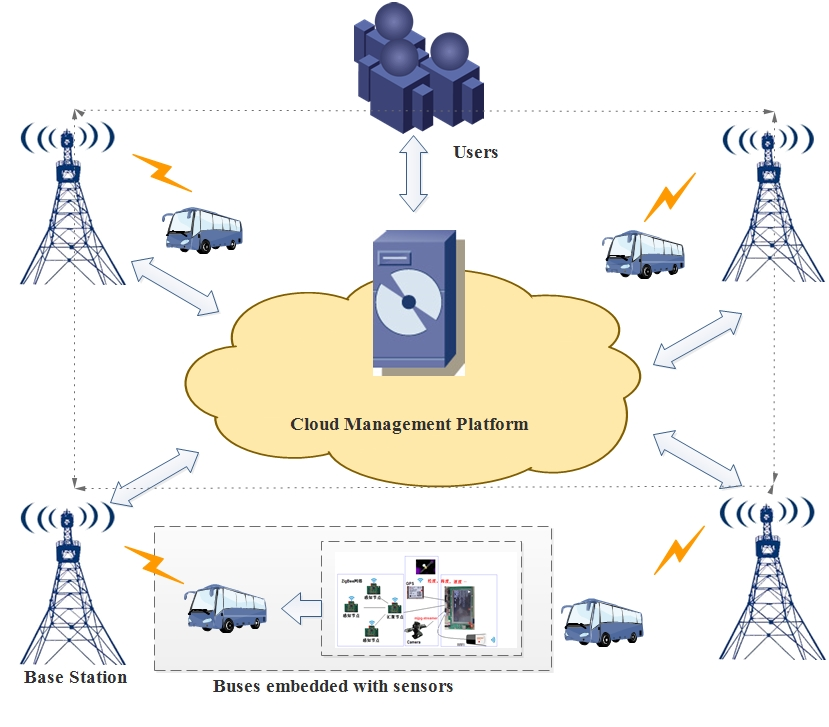
\includegraphics[width=1.0\linewidth]{Figure1.png}
	\caption[Fig.1]{An example of vehicle-based crowd sensing application. Buses embedded with plentiful sensors are distributed over a large city. Cloud management platform assign sensing task to the recruited vehicle which can contribute to the sensing tasks by returning their sensed data to CMP. And then CMP processes the received data to provide to user.}
	\label{Figure1}
\end{figure}

In this paper, we concentrate on how to achieve a high quality of crowd sensing making full use of the predictable location of buses. After an analysis on the relations between spatial-temporal coverage and the location of vehicle, we formulate the problem of selection vehicle (SV) for maximizing the spatial-temporal coverage of city with constraint budget. Through thoroughly proof, we find that SV is NP-hard. And we design a truthful and efficient approximation algorithm, called ECQA, to select a set of vehicle from all candidates under operation with a high efficiency (minimal budget and maximizing spatial-temporal coverage), which can approximate the optimal solution within a guarantee performance no less than $\left ( 1-e^{-1} \right )$, with polynomial-time computation complexity. We also theoretically prove the ECQA guarantee is truthfulness.


\section{SYSTEM MODEL AND PROBLEM FORMULATION}
\subsection{System Model }
We consider a vehicle-based crowd sensing system consisting of a CMP and many vehicles embedded with substantial sensors. The CMP periodically propagates sensing tasks to be completed by running vehicle. 
In a city area, we divide road into a serial of small segments. As an example shows in figure 2. Let $R$ denote the set of all small segments, $R=\left \{ r_{1},r_{2},r_{3},...,r_{k} \right \}$. When the CMP broadcasts a crowd-sensing task to be finished for a period of time, i.e. $T$. Supposed the time is discrete, so we can assume $T=\left \{ t_{1},t_{2},t_{3},...,t_{m} \right \}$.The distribution of vehicle is large-scale, each vehicle equipped with the sensor module that we has designed in [14] is able to join crowd-sensing tasks. Assume there are n vehicles can perform sensing assignments and the set of vehicles is denoted by $V=\left \{ v_{1},v_{2},v_{3},...,v_{n}\right \}$ . Initially, the CMP predicts the current position of all vehicles according to the timetable and broadcast the data packet until receive the ACK, if the prediction is not consistent with the actual current location obtained through Global Positioning System (GPS) [15] employed in vehicle, it will be updated, respectively.  With the initial location of vehicles and scheduled timetable, we can get the location of a vehicle $v_{i}$ at a specific time  $t_{j}$, which is denoted by  . Thus the trajectory of n vehicles can be represented as follows:
\setcounter{equation}{0}
\begin{equation}
L(V)=\begin{bmatrix}
l_{1}(t_{1})&l_{1}(t_{2})&... & l_{1}(t_{m})\\ 
l_{2}(t_{1})&l_{2}(t_{2})&... & l_{2}(t_{m})\\
.&. &.&.\\ 
.&. &.&.\\
.&. &.&.\\
l_{n}(t_{1})&l_{n}(t_{2})&... & l_{n}(t_{m})\\
\end{bmatrix}
\end{equation}
where the size of $L(V)$ is $n\times m$.


In practice, we are not anticipate that all vehicles are involved in crowd sensing due to it will introduce redundancy. For example, in terms with traffic monitoring, nearby vehicles usual upload the same traffic information, which ought to avoid. Therefore, we regular that a vehicle who is selected to take part in crowd sensing will gain a reward paid by CMP and the budget of CMP is limited and no morn than $C_{max}$. Next, we define the sensing reward.

\noindent
\textbf{Definition 1: Sensing Reward (SR)} a vehicle is selected to complete tasks often associated with a reward paid by CMP. Let $c_{i}$ denote the reward to $v_{i}$, the reward can be acquired through online bidding [1]. Then, the reward vector $C$ for all vehicles is:
\begin{equation}
\textbf{C}=\left \{c_{1},c_{2},...,c_{n} \right \}
\end{equation}
With the constraint of budget of CMP, not all vehicles participate in crowd-sensing, we utilize an indication vector $\Phi $ to imply whether a vehicle $v_{i}$ is selected or not
\begin{equation}
\Phi_{i}= \left\{\begin{matrix}
1&v_{i}\in \Omega \\ 
0&otherwise\end{matrix}\right.
\end{equation}

where $\Omega \subseteq V$ is the set of selected vehicles. Let $C$ be the total reward to buses in $\Omega$, which can be computed as
\begin{equation}
C(\Omega )=\left [ C,\Phi  \right ]
\end{equation}

As mentioned, the quality of crowd sensing is related with spatial-temporal coverage, which means to cover as many regions of interest as possible and ensure each road segment to be covered once at least within a sensing time $T$. Let we introduce the notion of spatial-temporal coverage.

\noindent
\textbf{Definition 2: Spatial-temporal Coverage (STC)} determines the quality of crowd-sensing. Formally, which can be defined as
\begin{equation}
\textbf{STC}=\sum_{t_{j}\in T}\bigcup_{v_{i}\in \Omega}\left (l_{i}(t_{j}) \right)
\end{equation}
Next, we show an example to explain the implication of STC. In Fig.2, the scheduled trajectory of Bus1, Bus2, Bus3, Bus4 is {BC, AB, AD,DE }, {BC BE, EH}, {EH, HD, AD, AB, BE},{EF, BE,AB, AD, DH}, respectively. In a period time $t_{1},t_{2},t_{3},t_{4}$ the location of  Bus1 to Bus4 is {BC, AD, DE, BC}, {BC, BE, BC,BE },{EH, HD, AB, BE}, {AB, BE, AD ,DH}, respectively. From equality $(1)$, we get
\begin{equation}
L(V)=\begin{bmatrix}
BC &AD &DE &BC \\ 
BC& BE &BC &BE\\ 
AB& BE &AB &BE\\ 
AB& BE &AD &DH
\end{bmatrix}
\end{equation}

If the CMP with budget limited is capable of selecting two vehicles to participate crowd-sensing, then we consider two cases as bellows
\begin{equation}
\begin{aligned}
STC({Bus1,Bus2})=& \underset{t_{1}}{\underbrace{BC}}+\underset{t_{2}}{\underbrace{AD+BE}}+\underset{t_{3}}{\underbrace{DE+BC}}\\&+\underset{t_{4}}{\underbrace{BC+BE}}
\end{aligned}
\end{equation}
\begin{equation}
STC({Bus3,Bus4})= \underset{t_{1}}{\underbrace{AB}}+\underset{t_{2}}{\underbrace{BE}}+\underset{t_{3}}{\underbrace{AB+AD}}+\underset{t_{4}}{\underbrace{BE}}
\end{equation}

It can be seen that the set of {Bus1, Bus2} have covered five different place in space and the segment of {BC} has been covered triple over time. On the contrary, the set of {Bus3, Bus4} simply have covered four different place in space, so we are more willing to select {Bus1, Bus2} to participate in crowd sensing.
\begin{figure}[t]
	\centering
	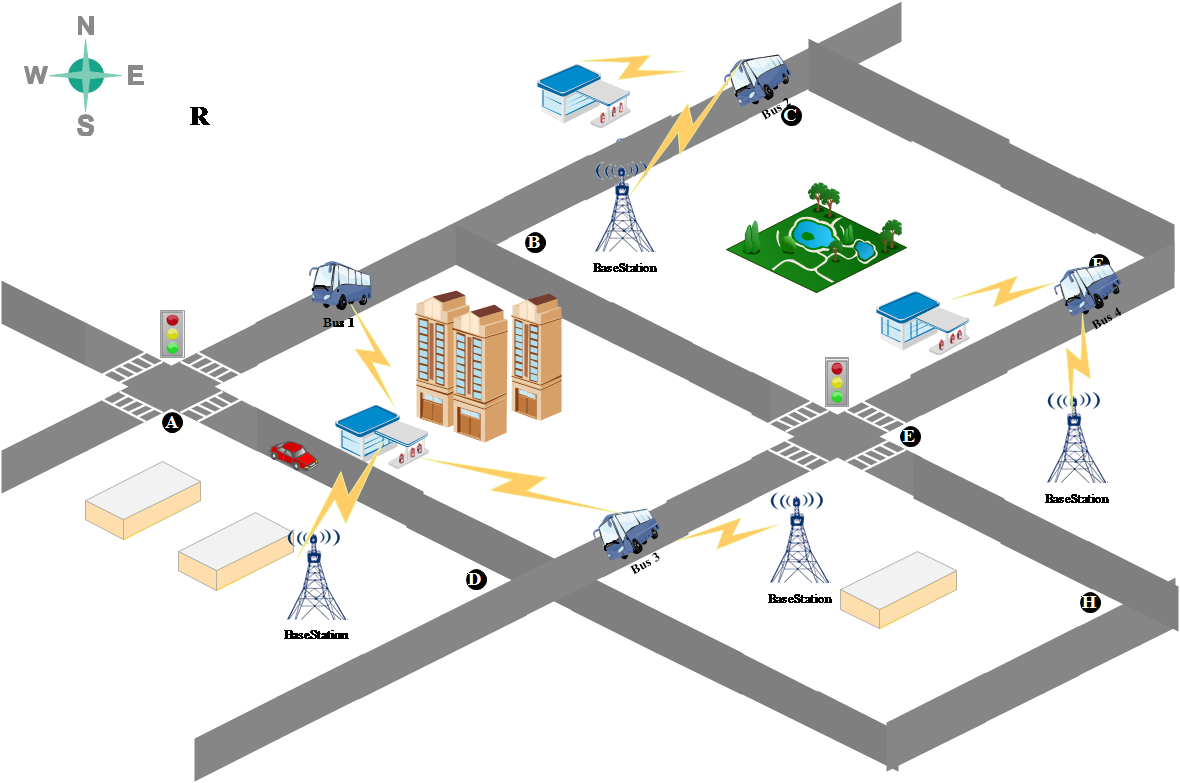
\includegraphics[width=1\linewidth]{Fig2.png}
	\caption{An example shows that we divide the city area into small fragments, such as $R =\left \{ AB, AD, BC, BE, DE, EF, EH, DH, CF \right \}$, where $R$ is the city area.}
	\label{fig:figure4}
\end{figure}	
\subsection{Problem Statement} 
In a region of interest, each vehicle equipped with amount of sensors which continuously sense the surrounding environment as it passes. However, at a specific moment, if all vehicles within a same road segment are involved in crowd-sensing, it will lead to overlap coverage. Thus it is highly demand to select an appropriate set to finish the crowd-sensing tasks and ensure the quality of crowd-sensing. Based on the system model, we are ready to formally define the problem of optimal selection of vehicle (SV) for maximizing the spatial-temporal coverage with SR budget constraint.	

\noindent
\textbf{Definition 3: SV Problem (SVP)}is to determine a set of vehicle under the budget constraint $C_{max}$ with the objective of maximizing the spatial-temporal coverage.
\begin{equation}
\begin{matrix}
\textbf{max}STC(\Omega ))\\\quad\quad\
\textbf{s.t.}\quad C(\Omega)\leqslant C_{max}\end{matrix}
\end{equation}

Actually, the sensing data at different road segment and at a different period time may have varying importance degree, such as we are more interested in hotspot with high traffic flow in the morning rush hour. For this reason, we introduce priority power to indicate the relative importance of each road segment where the higher priority a vehicle is more likely to be selected to join in crowd-sensing. Through analyzing historical data, it is easy to acquire traffic performance index (TPI) of each road segment. Let $D_{t_{j}}^{l_{i}}$ denote the TPI of $l_{i} (t_{j})$ at a specific time $t_{j}$, which is assumed known and normalized between 0 and 1, e.g. $D_{t_{j}}^{l_{i}}\in (0,1]$. With the TPI we define priority power.

\noindent
\textbf{Definition 4: Priority Power (PP)} is the importance of a road segment in a crowd-sensing period time, which is a function of  $D_{t_{j}}^{l_{i}}$ defined as $W_{t_{j}}^{l_{i}}(D_{t_{j}}^{l_{i}})$. So $D_{t_{j}}^{l_{i}}\propto W_{t_{j}}^{l_{i}}$, thus the first order derivative of $W_{t_{j}}^{l_{i}}(D_{t_{j}}^{l_{i}})$ satisfies
\begin{equation}
\frac{\mathrm{d}W_{t_{j}}^{l_{i}} }{\mathrm{d}D_{t_{j}}^{l_{i}}}> 0
\end{equation}
Therefore, priority power is expressed as follows
\begin{equation}
W_{t_{j}}^{l_{i}}=\log_{2}(1+D_{t_{j}}^{l_{i}})
\end{equation}
With the priority power, the STC can be redefined as
\begin{equation}
\sigma (\Omega )=\sum_{t_{j}\in T}\bigcup_{v_{i}\in \Omega }(l_{i}(t_{j})\cdot W_{t_{j}}^{l_{i}})
\end{equation}
so the SVP can be rewritten as
\begin{equation}
\begin{matrix}
\textbf{max}\  \sigma(\Omega)\\\quad\quad\quad\;\;\
\textbf{s.t.}\quad C(\Omega)\leqslant C_{max}\end{matrix}
\end{equation}

We hope that the solution of SVP can be found with a time efficient, unfortunately, it is NP-hard even though the trace of vehicles is predictable. In the next, we will prove SVP is NP-hard and propose an improved approximation algorithm based on greedy to solve it.
\section{SOLUTION TO THE SVP}
\subsection{Complexity Analysis of SVP}
Theorem 1. The SVP is NP-hard even though the trajectory of all vehicles are predictable.
Proof: To prove the NP-hard property of SVP, we should demonstrate it belongs to NP firstly, and then find another NP-hard problem proven that could be reduced to it. Assuming there is a possible solution $\Omega^{'}$, it is clearly that the correctness of this solution can be certified in polynomial, the time complexity of the checking algorithm is $O(n)$, which means SVP is NP. Next, we use an instance of budget maximum coverage problem as the known NP-hard, which is defined as follow. Given a collection of sets $S=\left \{S_{1},S_{2},...,S_{n}\right \}$, each set $S_{i}\subseteq R=\left \{ r_{1},r_{2},...,r_{m} \right \},i=1,2,3...,n$ has a cost  and an element $r_{j},j=1,2,3...m$ in R associated with a weight $w_{i}$.The question is whether we can find a subset  $S^{'}\subseteq S$ that the total cost is not more than a given budge $L$ and the total weight of elements in $S^{'}$ is maximized. Obviously, each set $S_{i}$ can be mapped to $\sigma(Z),Z\subseteq V,c_{i}$ be equivalent to $C(Z)$, and weight $w_{i}$ of each element in R is mapped to the priority power, $W_(t_{j})^(l_{i})$ of each vehicle in V. We have mapped the formulation of SVP to budget maximum coverage problem. And then we can see that a solution of budget maximum coverage problem is also the solution of SVP. So SVP is NP-hard.

Consequently, to achieve a truthful and computationally efficient crowd sensing system, it is highly demand to propose an approximate algorithm for solving SVP.
\subsection{Approximate Algorithm to Solve SVP}
We have analyzed the NP-hardness of SVP, it becomes computationally impracticable to select an optimal set of vehicles from all the candidate vehicles when the number of candidate vehicles is huge. As for a metropolis like Beijing, the number of vehicles under operations is about 30,000 by the end of 2016 [16]. To achieve the desired computational efficiency, we propose an approximate algorithm called efficient combination query algorithm (ECQA) to solve SVP. While designing the algorithm, not only should we consider to select a vehicle with maximized STC, but also ask for less reward from CMP with budget constraint. Therefore we define the reward efficient.

\noindent
\textbf{Definition 5: Reward Efficient (RE)} indicates the marginal STC achieve per unit reward.

The ECQA adopts a greedy strategy to solve the problem. The greedy policy is to select the next most reward effectiveness vehicle, which means to select a vehicle maximized marginal STC per unit reward, until the total SR exceed the budget of CMP. Mathematically, the reward-efficient for selecting a vehicle $v_{i}$ can be computed as follows
\begin{equation}
E_{i}=\frac{\sigma (\Omega ^{'}-\sigma (\Omega))}{c_{i}}
\end{equation}
The algorithm tries many rounds, a best vehicle with maximum RE is determined as a result of each round. In equation (14), where $E_{i}$  denotes the reward efficient of vehicle $v_{i}, Ω$ is solution obtained from $V, \Omega ^{'}=\left \{ \Omega\cup v_{i}  \right \}$ and $v_{i}\in V-\Omega $. The algorithm will not terminate until the budget constraint is active. The pseudo-code is listed in table 1.

\floatname{algorithm}{The pseudo-code of ECQA}
\renewcommand{\algorithmicrequire}{\textbf{Input:}}
\renewcommand{\algorithmicensure}{\textbf{Output:}}
\begin{algorithm}
	\caption{}	
	\begin{algorithmic}
		\Require set $V=\left \{  v_{1},v_{2},v_{3},...,v_{n}\right \}$ of vehicle under operation, set S$C=\left \{  c_{1},c_{2},c_{3},...,c_{n}\right \}$ sensing reward of each vehicle, $C_{max}$ the budget constraint of CMP, an initial set $S^{0}$ of cardinality is an integer as 3, assume the schedule time of each vehicle is known.
		\Ensure set $\Omega $ is the best set of vehicle selected by ECQA. 
		\State $max \gets 0$
		\State $\Omega \gets \varnothing$
		\State $S \gets \varnothing$
		\For{$S^{0}\subseteq V,C(S^{0})\leqslant C_{max}$}
			\State $S \gets S^{0}$
			\For{$v_{i}\in V-S$}
				\State $S^{'} \gets \left \{ S\cup v_{i} \right \}$
				\State $E_{i} \gets \frac{\sigma(S^{'})-\sigma (S)}{c_{i}}$
				\If{$E_{i}>max\quad \textbf{and}\quad C(S^{'})<C_{max}$}
					\State $S \gets S^{'}$
					\State $max \gets E_{i}$
				\EndIf
				\If{$\sigma(S)>\sigma()\Omega)$}
					\State $ \sigma \gets S$
				\EndIf
			\EndFor		
		\EndFor				
	\end{algorithmic}
\end{algorithm}


The ECQA has a performance guarantee $ \rho \leqslant 1$, which indicates we can obtain a solution is $\rho$ times of optimal solution in NP-hard problem [17]. The closer of value of $\rho$ to 1, the more approximation to optimal solution. In this paper, the ECQA can achieve a lower bound ratio of  $\left (1-e^{-1}  \right )$ when the cardinality as $q$ of set $S^{0}$ is not less than three, i.e. $q\geqslant 3$. Next, we will prove the following theorem about the performance guarantee of ECQA.

\noindent
\textbf{Theorem 2.} The ECQA can achieve a worst performance guarantee of  $\left (1-e^{-1}  \right )$ for $\left |q\geqslant 3 \right|$. 
\begin{equation}
\sigma (\Omega )\geqslant \left (1-e^{-1}  \right )\cdot \sigma (Opt), q\geqslant 3
\end{equation}
where $Opt$ is the set in an optimal solution.

\noindent
\textbf{Proof:} Let’s redefine $v_{i}\in V,i=1,2,3,...,r$ as a vehicle added into $\Omega$ in i-th iteration, Let $\Omega_{k}$ denote $ \bigcup_{i=1}^{k}v_{i}$, and $\Omega =\Omega _{r}$. To prove inequality (15), the following two inequalities we can derive from [18], After $i,i=1,2,3,...,r+1$ iterations, we can get
\begin{equation}
\sigma (\Omega _{i})\geqslant \left [ 1-\coprod_{m=1}^{i}(1-\frac{c_{m}}{C_{max}}) \right ]\cdot \sigma (Opt)
\end{equation}
\begin{equation}
\begin{aligned}
\sigma (\Omega _{r+1})&\geqslant \left [ 1-\coprod_{m=1}^{r+1}(1-\frac{c_{m}}{C_{max}}) \right ]\cdot \sigma (Opt) \\ & \geqslant \left [ 1-\left ( 1-\frac{1}{r+1} \right )^{r+1} \right ]\cdot\sigma (Opt)\\&\geqslant \left (1-e^{-1}  \right )\cdot\sigma (Opt) 
\end{aligned}
\end{equation}
where $c_{m}$ denotes the sensing reward to $v_{m}$. The detailed proof of inequalities (16), (17)can be found in [17],[18]. We can easily to know that (17) is equivalent to following inequality
\begin{equation}
\begin{aligned}
\sigma (\Omega _{r+1})=\sigma(\Omega _{r})+\sigma(\left \{ v_{r+1}\right \})\geqslant\left ( 1-e^{-1} \right ) \cdot \sigma (Opt)
\end{aligned}
\end{equation}
where $v_{r+1}$ is selected at $r+1$ round but not added to $\Omega$ due to overflow budget constraint $C_{max}$. Applying (16) to (18), we get
\begin{equation}
\sigma (\Omega _{r}-S^{0})+\sigma (\left \{ v_{r+1} \right \})\geqslant \left ( 1-e^{-1} \right )\cdot \sigma (Opt-S^{0})
\end{equation}
where the set $Opt-S^{0}$ means that an element belongs to set Opt but not in set $S^{0}$.

Assuming $\sigma\left(\left \{ v_{r+1} \right \}\right)$ is greater than $\sigma\left ( \left \{ v_{i} \right \} \right),i=1,2,3,...,r$, if this were the case, $v_{r+1}$ is bound to be selected before $v_{i}$ and included in $\Omega _{r}$, so this assumption is invalid. Therefore, we can get
\begin{equation}
q\cdot \sigma \left ( \left \{ v_{r+1} \right \} \right )\leqslant \sigma \left ( S^{0} \right )
\end{equation}
From (19), (20) the following inequality can be hold
\begin{equation}
\sigma \left ( \Omega _{r} \right )\geqslant \left ( 1-e^{-1} \right )\cdot \sigma (Opt-S^{0})+(1-q^{-1})\cdot \sigma (S^{0})
\end{equation}
where e is a natural base whose value is less than three, hence
\begin{equation}
\sigma \left ( \Omega _{r} \right )\geqslant \left ( 1-e^{-1} \right )\cdot (\sigma (Opt-S^{0})+\sigma (S^{0}))
\end{equation}
if and only if $q\geqslant 3$, the inequality (21) makes sense. Clearly, $\sigma(Opt-S^{0})+\sigma (S^{0})=\sigma (Opt)$, and then
\begin{equation}
\sigma(\Omega_{r})\geqslant (1-e^{-1})\cdot (Opt), \ for \ q\geqslant 3
\end{equation}

Owing to the final output of ECQA as good as $\Omega_{r}$ if not better, this prove the performance guarantee of $(1-e^{-1})$.


\section{EVALUATION}
Extensive simulations has been conducted to evaluation the performance of our proposed algorithm. The traffic trace dataset we used, the simulation setup, the compared algorithms, and the performance comparison and discussion are presented as follows.


\subsection{Real Traffic Trace Used and Simulation Setup}
In our simulation, to make the evaluation results convincing, the T-Drive trajectory dataset [19], [20] that contains a one-week trajectory of 10,357 buses. The total number of points in this dataset is about 15 million and the total distance of the trajectories reaches 9 million kilometers. We have imported the processed data into the Google Global Mapper, as Fig.3 shows, the distribution of the trajectories of vehicles basically covers the whole traffic network of Beijing. Our simulation are performed on traces extracted from the dataset on February 3, 2008, 6 AM to 10 PM. We randomly extract a small number of vehicles from processed dataset to participate in crowd-sensing, i.e., 10, so that the optimal solution can be found though an enumeration algorithm. Each vehicle is associated with a SR, and the SR of a vehicle is uniformly distributed in [0.7, 1.2].   
\subsection{Algorithm in Comparison}
The quality of crowd-sensing is related to STC, we evaluation how the total sensing reward $C_{max}$, the number of time period m, and the initial size of solution q impact on the performance. In this paper, we compare the performance of our algorithm with two baseline algorithm. 1) The enumerative algorithm (EA) can always get the optimal vehicles from the candidate vehicles by exhaustive search, however, the SVP is NP-hard, when the number of candidate vehicles is larger, it becomes infeasible to obtain the optimal solution in polynomial time. Thus, the EA is applied simply when the number of vehicles is small. 2) The simulated annealing algorithm (SAA) is often used to solve optimization problems, we improve a SAA to compute the SVP for maximizing the STC. Furthermore, the results are also compared with the lower bound performance guarantee STC $EA\cdot(1-e^{-1})$.

\begin{figure}
	\centering
	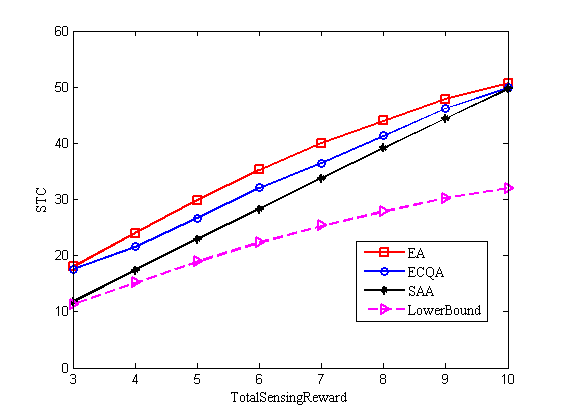
\includegraphics[width=1\linewidth]{Fig4(a).png}
	\caption{The total sensing reward $C_{max}$ is [3,10], the initial size of solution is 3, the number of period time is 6.}
	\label{fig:figure4}
\end{figure}
\begin{figure}
	\centering
	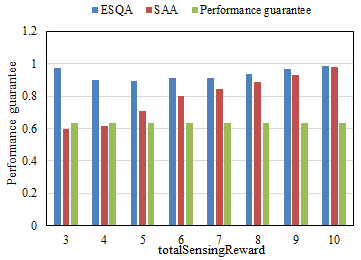
\includegraphics[width=1\linewidth]{Fig4(b).png}
	\caption{The total sensing reward $C_{max}$ is [3,10], the initial size of solution is 3, the number of period time is 6.}
	\label{fig:figure6}
\end{figure}
\begin{figure}
	\centering
	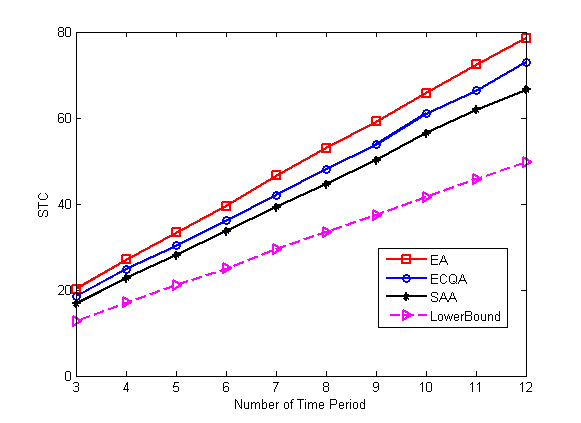
\includegraphics[width=1\linewidth]{Fig4(c).png}
	\caption{ The number of period is [4, 12], the total sensing reward $C_{max}$ is 6, the initial size of solution is 3.}
	\label{fig:figure5}
\end{figure}

\begin{figure}
	\centering
	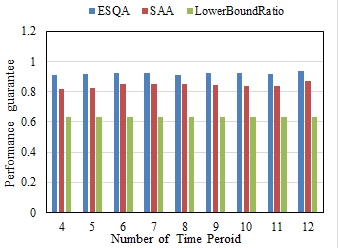
\includegraphics[width=1\linewidth]{Fig4(d).png}
	\caption{The number of period is [4, 12], the total sensing reward $C_{max}$ is 6, the initial size of solution is 3.}
	\label{fig:figure5}
\end{figure}

\begin{figure}
	\centering
	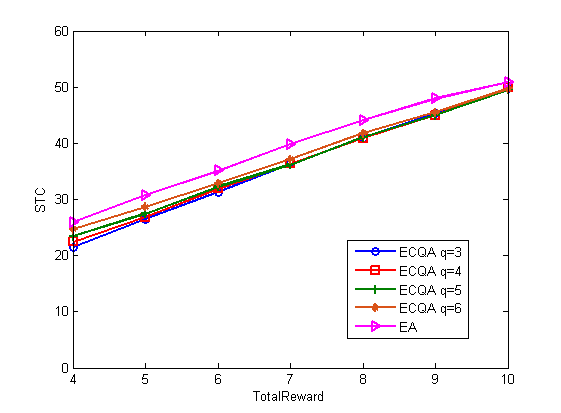
\includegraphics[width=1\linewidth]{Fig4(e).png}
	\caption{The initial size of solution is [3, 6], the total sensing reward is [4, 10], the number of period time is 6.}
	\label{fig:figure6}
\end{figure}


\begin{figure}
	\centering
	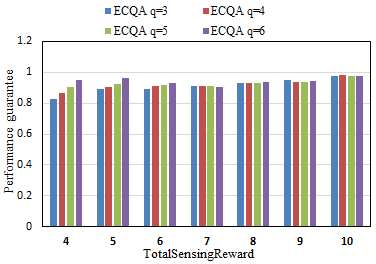
\includegraphics[width=1\linewidth]{Fig4(f).png}
	\caption{The initial size of solution is [3, 6], the total sensing reward is [4, 10], the number of period time is 6.}
	\label{fig:figure5}
\end{figure}
Figs.4 illustrate the performance during the variation of the total sensing reward $C_{max}$, the number of period time $m$ and the initial size of solution $q$. In this group of simulation, we extract 10 vehicles from dataset. From Figs.3 to Figs.8 , we can observe the truth that the algorithm which is proposed in this paper outperforms the one with SAA, and gets closer to the optimal EA. In Fig.3, the STC of our algorithm is larger than the SAA, and if the total sensing reward is enough, the ECQA and EA tends to equal to optimal. The result fit in with reality. In Figs.4 (b), a very brighten evidence is revealed. The performance guarantee of ECQA fluctuates around 0.9 and still provide a performance guarantee larger than $EA\cdot(1-e^{-1})$ as we have proven. This result indicates that in real cases, our algorithm is more likely to achieve full-coverage and ensure the integrity of sensing data. Figs.4 (c) shows, along with the increase of the number of period time $m$, the STC of both ECQA and competitors become larger and larger. This is because the route of vehicle is scheduled cyclically movement, the larger number of period time, one segment may be covered many time as Fig.2 depicted. Additionally, the performance gap between ECQA and EA stayed nearly constant as $m$ and the performance guarantee is greater than 0.9 consistently as Fig.4 (d) shown. In Figs.4 (e) to (f), we study the important parameter $q$ influence on performance of ECQA, the $q$ is varied from 4 to 10. It is easy to see that, when total sensing reward is less than 7, the STC increase with $q$, otherwise is even nearly. This result can be understood since the total sensing reward is insufficient, the $q$ is larger, ECQA primarily searches a larger domain for optimal solution, but it takes longer execution time actually. In contract, $q$ has slightly impact on STC, which suggests that we can produce a good performance even with a small $q$ and spend less execution time simultaneously. 
\section{CONCLUTION}
In this paper, we introduce mobile crowd-sensing into vehicular network to produce a vehicle-based crowd sensing network. Due to the quality of crowd-sensing is extraordinarily sensitive to the location of participants, so we take full advantage of predictable mobility pattern of public transport buses which traveling route is scheduled. In this scenario, we need to address a crucial problem of the selection of vehicle to participate in urban sensing for maximizing spatiotemporal coverage. We have proven that the problem of selecting vehicles under a given constraint sensing reward for maximizing spatiotemporal coverage is NP-hard. Then we present the ECQA which aims to select an optimal vehicles collection for maximizing the spatiotemporal coverage by taking the current and future positions into account of each vehicle. Moreover, though the theoretical analysis and a series of simulation on real T-Drive trajectory dataset, we prove that the ECQA can achieve a performance guarantee is still greater than $(1-e^{-1})$ of optimum and obtain better performance than alternative algorithm.




% You must have at least 2 lines in the paragraph with the drop letter
% (should never be an issue)








% An example of a floating figure using the graphicx package.
% Note that \label must occur AFTER (or within) \caption.
% For figures, \caption should occur after the \includegraphics.
% Note that IEEEtran v1.7 and later has special internal code that
% is designed to preserve the operation of \label within \caption
% even when the captionsoff option is in effect. However, because
% of issues like this, it may be the safest practice to put all your
% \label just after \caption rather than within \caption{}.
%
% Reminder: the "draftcls" or "draftclsnofoot", not "draft", class
% option should be used if it is desired that the figures are to be
% displayed while in draft mode.
%
%\begin{figure}[!t]
%\centering
%\includegraphics[width=2.5in]{myfigure}
% where an .eps filename suffix will be assumed under latex, 
% and a .pdf suffix will be assumed for pdflatex; or what has been declared
% via \DeclareGraphicsExtensions.
%\caption{Simulation results for the network.}
%\label{fig_sim}
%\end{figure}

% Note that the IEEE typically puts floats only at the top, even when this
% results in a large percentage of a column being occupied by floats.


% An example of a double column floating figure using two subfigures.
% (The subfig.sty package must be loaded for this to work.)
% The subfigure \label commands are set within each subfloat command,
% and the \label for the overall figure must come after \caption.
% \hfil is used as a separator to get equal spacing.
% Watch out that the combined width of all the subfigures on a 
% line do not exceed the text width or a line break will occur.
%
%\begin{figure*}[!t]
%\centering
%\subfloat[Case I]{\includegraphics[width=2.5in]{box}%
%\label{fig_first_case}}
%\hfil
%\subfloat[Case II]{\includegraphics[width=2.5in]{box}%
%\label{fig_second_case}}
%\caption{Simulation results for the network.}
%\label{fig_sim}
%\end{figure*}
%
% Note that often IEEE papers with subfigures do not employ subfigure
% captions (using the optional argument to \subfloat[]), but instead will
% reference/describe all of them (a), (b), etc., within the main caption.
% Be aware that for subfig.sty to generate the (a), (b), etc., subfigure
% labels, the optional argument to \subfloat must be present. If a
% subcaption is not desired, just leave its contents blank,
% e.g., \subfloat[].


% An example of a floating table. Note that, for IEEE style tables, the
% \caption command should come BEFORE the table and, given that table
% captions serve much like titles, are usually capitalized except for words
% such as a, an, and, as, at, but, by, for, in, nor, of, on, or, the, to
% and up, which are usually not capitalized unless they are the first or
% last word of the caption. Table text will default to \footnotesize as
% the IEEE normally uses this smaller font for tables.
% The \label must come after \caption as always.
%
%\begin{table}[!t]
%% increase table row spacing, adjust to taste
%\renewcommand{\arraystretch}{1.3}
% if using array.sty, it might be a good idea to tweak the value of
% \extrarowheight as needed to properly center the text within the cells
%\caption{An Example of a Table}
%\label{table_example}
%\centering
%% Some packages, such as MDW tools, offer better commands for making tables
%% than the plain LaTeX2e tabular which is used here.
%\begin{tabular}{|c||c|}
%\hline
%One & Two\\
%\hline
%Three & Four\\
%\hline
%\end{tabular}
%\end{table}


% Note that the IEEE does not put floats in the very first column
% - or typically anywhere on the first page for that matter. Also,
% in-text middle ("here") positioning is typically not used, but it
% is allowed and encouraged for Computer Society conferences (but
% not Computer Society journals). Most IEEE journals/conferences use
% top floats exclusively. 
% Note that, LaTeX2e, unlike IEEE journals/conferences, places
% footnotes above bottom floats. This can be corrected via the
% \fnbelowfloat command of the stfloats package.








% if have a single appendix:
%\appendix[Proof of the Zonklar Equations]
% or
%\appendix  % for no appendix heading
% do not use \section anymore after \appendix, only \section*
% is possibly needed

% use appendices with more than one appendix
% then use \section to start each appendix
% you must declare a \section before using any
% \subsection or using \label (\appendices by itself
% starts a section numbered zero.)
%


\appendices

%Appendix one text goes here.

%% you can choose not to have a title for an appendix
%% if you want by leaving the argument blank


% use section* for acknowledgment
%\section*{Acknowledgment}

\section*{Acknowledgment}


This paper was supported by National Science and Technology Major Project (2016ZX03001012) and the State Major Science and Technology Special Projects of China under Grant 2016ZX03001017-004.
%The authors would like to thank...


% Can use something like this to put references on a page
% by themselves when using endfloat and the captionsoff option.
\ifCLASSOPTIONcaptionsoff
  \newpage
\fi



% trigger a \newpage just before the given reference
% number - used to balance the columns on the last page
% adjust value as needed - may need to be readjusted if
% the document is modified later
%\IEEEtriggeratref{8}
% The "triggered" command can be changed if desired:
%\IEEEtriggercmd{\enlargethispage{-5in}}

% references section

% can use a bibliography generated by BibTeX as a .bbl file
% BibTeX documentation can be easily obtained at:
% http://mirror.ctan.org/biblio/bibtex/contrib/doc/
% The IEEEtran BibTeX style support page is at:
% http://www.michaelshell.org/tex/ieeetran/bibtex/
%\bibliographystyle{IEEEtran}
% argument is your BibTeX string definitions and bibliography database(s)
%\bibliography{IEEEabrv,../bib/paper}
%
% <OR> manually copy in the resultant .bbl file
% set second argument of \begin to the number of references
% (used to reserve space for the reference number labels box)
\begin{thebibliography}{1}

\bibitem{IEEEhowto:kopka}
Zhu.Y, Bao.Y, Li.B. ``On Maximizing Delay-Constrained Coverage of Urban Vehicular Networks[J]." \textit{IEEE Journal on Selected Areas in Communications}, 2012, 30(4):804-817.

\bibitem{IEEEhowto:kopka}
Dejun Yang, Guoliang Xue, Xi Fang, and Jian Tang, ``Crowdsourcing to smart phones: incentive mechanism design for mobile phone sensing", in\textit{ACM MOBICOM}, 201. 

\bibitem{IEEEhowto:kopka}
Mohammad Nozari Zarmehri and Ana Aguiar, ``Supporting sensing application in vehicular networks", in\textit{ ACM CHANTS}, 2012

\bibitem{IEEEhowto:kopka}
E.Koukoumidis,L.S.Peh, M.R.Martonosi,``Signalguru:Leveraging mobile phones for collaborative traffic signal schedule advisory", in \textit{Proc. 9th Int. Conf. Mobile Syst., Appl. Serv., ACM}, 2011, pp. 127–140. 

\bibitem{IEEEhowto:kopka}
A. Thiagarajan et al., ``Vtrack: Accurate, energy-aware road traffic delay estimation using mobile phones",\textit{7th ACM Conf.Embedded Netw. Sensor Syst., ACM}, 2009, pp. 85–98.

\bibitem{IEEEhowto:kopka}
P. Dutta, P. M. Aoki, and et al., ``Common Sense: participatory urban sensing using a network of handheld air quality monitors," in \textit{SenSys 2009}, pp. 349–350.

\bibitem{IEEEhowto:kopka}
A.Farshad, M. K. Marina, and F. Garcia, ``Urban WiFi characterization via mobile crowdsensing," in \textit{Proc. Netw. Oper. Manage. Symp., IEEE}, 2014, pp. 1–9.

\bibitem{IEEEhowto:kopka}
Feng Z, Zhu Y, Zhang Q, et al. ``TRAC: Truthful auction for location-aware collaborative sensing in mobile crowdsourcing[C]" // \textit{INFOCOM, 2014 Proceedings IEEE.} IEEE, 2014:1231-1239.

\bibitem{IEEEhowto:kopka}
D. Yang, G. Xue, and et al., ``Crowdsourcing to smartphones: Incentive mechanism design for mobile phone sensing," in\textit{ MobiCom 2012}, pp. 173–184.

\bibitem{IEEEhowto:kopka}
S. Reddy, D. Estrin, M. Hansen, and M. Srivastava, ``Examining micropayments for participatory sensing data collections," in \textit{UbiComp 2010}, pp. 33–36.

\bibitem{IEEEhowto:kopka}
He Z, Cao J, Liu X. ``High quality participant recruitment in vehicle-based crowdsourcing using predictable mobility," \textit{Computer Communications. IEEE}, 2015:2542-2550.

\bibitem{IEEEhowto:kopka}
L. Kazemi and C. Shahabi, ``Geocrowd: Enabling query answering with spatial crowdsourcing," in \textit{ACM SIGSPATIAL 2012}, pp. 189–198.

\bibitem{IEEEhowto:kopka}
J. Huang and H.-S. Tan, ``Vehicle future trajectory prediction with a DGPS/INS-based positioning system," in \textit{American Control Conference}, 2006.

\bibitem{IEEEhowto:kopka}
 Kang L, Poslad S, Wang W, et al. ``A Public Transport Bus as a Flexible Mobile Smart Environment Sensing Platform for IoT" \textit{ International Conference on Intelligent Environments. IEEE, 2016}.
 
\bibitem{IEEEhowto:kopka}
 Rai A, Chintalapudi K K, Padmanabhan V N, et al. ``Zee:zero-effort crowdsourcing for indoor localization[C]"// 2012:293-304.
 
\bibitem{IEEEhowto:kopka}
\textit{https://baike.baidu.com/item}.

\bibitem{IEEEhowto:kopka}
 MAXIM S. ``A note on maximizing a sub-modular set function subject to knapsack constraint [ J]" . \textit{Operations Research Letters, 2004},32( 5): 41-43.
 
\bibitem{IEEEhowto:kopka}
Khuller S, Moss A, Naor J. ``The budgeted maximum coverage problem [M]".\textit{Elsevier North-Holland}.

\bibitem{IEEEhowto:kopka}
Jing Yuan, Yu Zheng, Xing Xie, and Guangzhong Sun. ``Driving with knowledge from the physical world." \textit{In The 17th ACM SIGKDD international conference on Knowledge Discovery and Data mining, KDD’11,} New York, NY, USA, 2011. ACM.

\bibitem{IEEEhowto:kopka}
Jing Yuan, Yu Zheng, Chengyang Zhang, Wenlei Xie, Xing Xie, Guangzhong Sun, and Yan Huang. ``T-drive: driving directions based on taxi trajectories". \textit{In Proceedings of the 18th SIGSPATIAL International Conference on Advances in Geographic Information Systems,} GIS ’10, pages 99-108, New York, NY, USA,2010. ACM.
%\bibitem{IEEEhowto:kopka}
%S. W. Jeon, K. Kim, J. Yang and D. K. Kim, "The Feasibility of Interference Alignment for MIMO Interfering Broadcast—Multiple-Access Channels," IEEE Trans. Wireless Commun., vol. 16, no. 7, pp. 4614-4625, Jul. 2017.

\end{thebibliography}

% biography section
% 
% If you have an EPS/PDF photo (graphicx package needed) extra braces are
% needed around the contents of the optional argument to biography to prevent
% the LaTeX parser from getting confused when it sees the complicated
% \includegraphics command within an optional argument. (You could create
% your own custom macro containing the \includegraphics command to make things
% simpler here.)
%\begin{IEEEbiography}[{\includegraphics[width=1in,height=1.25in,clip,keepaspectratio]{mshell}}]{Michael Shell}
% or if you just want to reserve a space for a photo:



% You can push biographies down or up by placing
% a \vfill before or after them. The appropriate
% use of \vfill depends on what kind of text is
% on the last page and whether or not the columns
% are being equalized.

%\vfill

% Can be used to pull up biographies so that the bottom of the last one
% is flush with the other column.
%\enlargethispage{-5in}



% that's all folks
\end{document}


